% =============================================================================
% IT-Innovation -- Zweiseitige Zusammenfassung der Masterarbeit
% Eigenstaendig kompilierbar:  pdflatex zusammenfassung.tex  (zweimal)
% =============================================================================
\documentclass[11pt,a4paper,twocolumn]{scrartcl}

\usepackage[utf8]{inputenc}
\usepackage[T1]{fontenc}
\usepackage[ngerman]{babel}
\usepackage{lmodern}
\usepackage[protrusion=true,expansion=true]{microtype}
\usepackage[a4paper,left=1.6cm,right=1.6cm,top=1.8cm,bottom=1.6cm,columnsep=0.7cm]{geometry}
\usepackage{booktabs}
\usepackage{tabularx}
\usepackage{enumitem}
\usepackage{graphicx}
\usepackage{float}
\usepackage{subcaption}
\usepackage{caption}
\captionsetup{font=small,labelfont=bf}
\graphicspath{{../thesis/images/}}
\usepackage{cleveref}
\crefname{figure}{Abb.}{Abb.}
\Crefname{figure}{Abbildung}{Abbildungen}

\setlength{\parskip}{0.12em}
\setlength{\parindent}{0pt}
\setlength{\intextsep}{4pt plus 2pt minus 2pt}
\setlength{\textfloatsep}{5pt plus 2pt minus 2pt}
\setlength{\dbltextfloatsep}{4pt plus 2pt minus 2pt}
\setlength{\abovecaptionskip}{3pt}
\setlength{\belowcaptionskip}{0pt}

% Einheitliche, kompakte Abstaende fuer alle Sections
\RedeclareSectionCommand[beforeskip=-1.0em, afterskip=0.4em]{section}

\begin{document}
\pagestyle{empty}
\thispagestyle{empty}
\raggedbottom

\twocolumn[{%
\begin{center}
  {\LARGE\bfseries Prognose individuellen Mobilit\"atsverhaltens auf Basis\\[0.2em]
   eines mit Bewegungsdaten trainierten Machine-Learning-Modells\par}
  \vspace{0.9em}
  \begin{tabular}{c@{\hspace{3em}}c@{\hspace{3em}}c}
    {\large Achim Baumgärtner} & {\large Gian Ledl-Truöl} & {\large Prof.\,Dr.\ Sonntag} \\[0.15em]
  \end{tabular}\par
  \vspace{0.4em}
  {\small Fakultät Informatik und Informationstechnik, Hochschule Esslingen\par}
\end{center}
\vspace{0.3em}
}]
\vspace{-0.8em}

\section{Motivation und Problemstellung}

Elektrofahrzeuge gelten als mobiler Stromspeicher und genau diese Eigenschaft macht sie für die Energiewende interessant. Um Strom, der zu einem bestimmten Zeitpunkt überschüssg ist, speichern zu können, benötigt man Akkumulatoren. Bidirektionales Laden, kurz Vehicle-to-Grid (V2G), macht das technisch möglich: Ein Elektrofahrzeug gibt Energie ans Netz ab, wenn es lädt und über genügend Energie verfügt, wenn weniger Strom erzeugt wird, als verbraucht wird. Dieses Potenzial bleibt jedoch weitgehend ungenutzt, solange nicht bekannt ist, \emph{wann} ein Fahrzeug in den nächsten Tagen gefahren wird und wann es dem Netz zur Verfügung steht.

Genau hier setzt diese Arbeit an. Das Ziel ist ein Machine-Learning-Modell, welches das individuelle Nutzungsverhalten eines Elektrofahrzeugs zuverlässig prognostizieren kann. Das heißt konkret: stündlich, über einen Horizont von bis zu sieben Tagen. Die zentrale Herausforderung dabei ist nicht algorithmischer, sondern datenseitiger Natur. Individuelles Fahrverhalten ist stark heterogen~\cite{ji2023rethinking}: Ein Pendler fährt täglich potentiell zur selben Zeit, ein Gelegenheitsfahrer völlig unregelmäßig. Ein einziges, übergreifendes Modell kann dieser Varianz kaum gerecht werden -- was sowohl die Modellwahl als auch die Frage nach der Datengrundlage stark beeinflusst.

Hinzu kommt, dass für individuelle Fahrzeugnutzungsdaten kein etabliertes Standardformat existiert. Datensätze aus verschiedenen Studien unterscheiden sich erheblich in Schema und Granularität: Manche enthalten nur Zeitstempel und einen binären Fahrzustand, andere zusätzlich physikalische Größen wie Energieverbrauch, Ortsdaten oder Batteriespannung. Eine direkte Vergleichbarkeit ist damit von vornherein nicht gegeben, was den Umgang mit realen Mobilitätsdaten zu einer eigenständigen methodischen Aufgabe macht.

\section{Forschungsfragen}
\label{sec:forschungsfragen}

Aus dem Vorangegangenen stellen sich nun die folgenden Forschungsfragen, die die Arbeit strukturieren. 

Erstens: Welche Verfahren des überwachten Lernens eignen sich zur Prognose des individuellen Mobilitätsverhaltens, und wie genau lassen sich Abfahrts- und Rückkehrzeiten über bis zu sieben Tage vorhersagen? Zweitens: Welchen Einfluss hat die Datenquelle selbst auf die Prognosegüte -- unabhängig vom gewählten Algorithmus? Und drittens: Welche Merkmale, etwa Tageszeit oder Wochentag, tragen am stärksten zur Vorhersagequalität bei?
In bestehenden Studien werden Datenqualität und Algorithmuswahl häufig gemeinsam variiert, was eine saubere Ursachenzuschreibung verhindert. Diese Arbeit hält den Algorithmus bewusst konstant und variiert nur die Datenquelle, was dazu führt, dass der Effekt der Datenbasis isoliert werden kann.

\section{Daten und Methodik}

Die Datengrundlage setzt sich aus fünf Quellen zusammen: synthetische emobpy-Profile~\cite{gaetemorales2020emobpy}, reale EV-Felddaten eines Audi e-tron~\cite{pozzato2023fielddata}, das Vehicle Energy Dataset (VED)~\cite{oh2020ved}, eine regelbasierte Routine-Zeitreihe als kontrollierbarer Referenzfall sowie -- als bewusster Kontrast ohne Fahrzeugbezug -- die menschlichen Bewegungsdaten YJMob100K~\cite{yabe2024yjmob}, bei denen ein Aktiv-Label aus Standortwechseln abgeleitet wird. Die bewusst heterogene Auswahl dient dazu, Aussagen über die Robustheit der Modelle zu ermöglichen, die über einen einzelnen Datensatz hinausgehen.

Da die Quellformate nicht kompatibel sind, überführt ein Adapter alle Datensätze in ein einheitliches Schema (\texttt{vehicle\_id, timestamp, driving}) mit stündlicher Auflösung. Die weitere Verarbeitung folgt einer festen Pipeline (\cref{fig:pipeline}): Bereinigung fehlerhafter Werte, Anonymisierung personenbezogener Merkmale, anschließendes Feature Engineering. Abgeleitet werden Kalendermerkmale (Stunde, Wochentag, Feiertag), Lag-Merkmale (lag\textsubscript{1}, lag\textsubscript{2}, lag\textsubscript{24}, lag\textsubscript{168}) sowie rollierende Mittelwerte über 24 und 168 Stunden. Die Lags respektieren dabei strikt die Fahrzeuggrenzen, um Datenlecks zu verhindern.

\begin{center}
  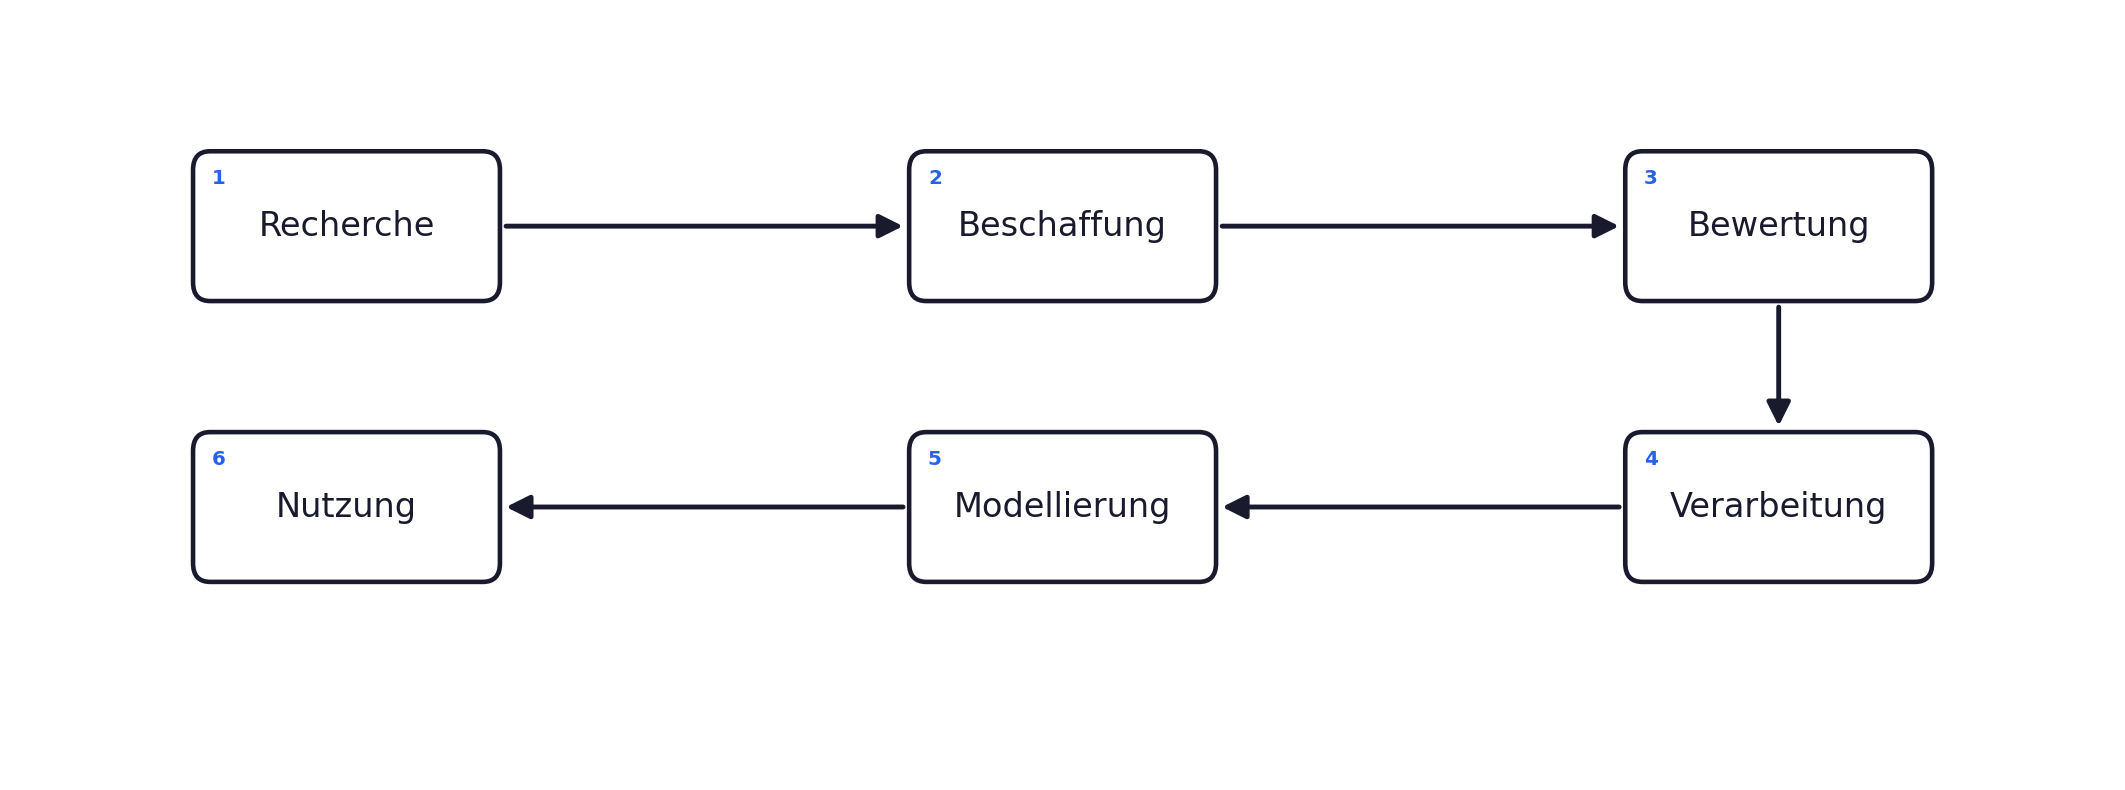
\includegraphics[width=0.88\columnwidth]{prozess_diagramm.png}
  \captionof{figure}{Verarbeitungs-Pipeline: von der Rohdatenquelle bis zur Modellnutzung.}
  \label{fig:pipeline}
\end{center}

Als Lernverfahren kommen baumbasierte Ensemble-Methoden (\cref{fig:tree}) zum Einsatz: Random Forest~\cite{breiman2001random} als interpretierbare Baseline sowie Gradient Boosting (LightGBM) als leistungsfähigeres Verfahren. Die Aufgabe ist eine binäre Klassifikation aus der sich Abfahrts- und Rückkehrzeiten ableiten lassen. Die zwei Klassen sind Fahr- und Standzeit, wobei die Fahrzeit als positive Klasse definiert ist.

\begin{center}
  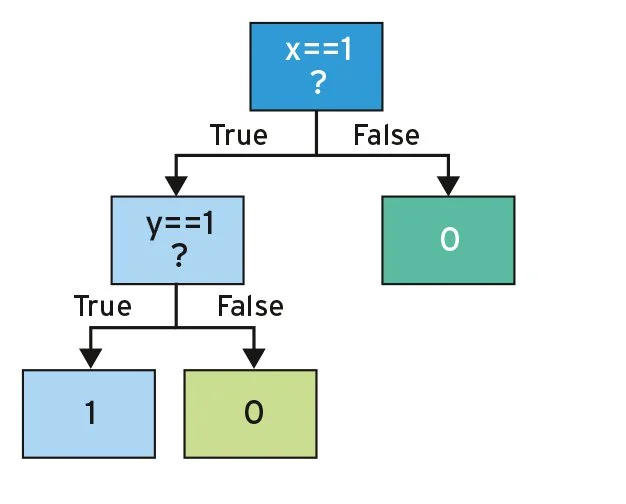
\includegraphics[width=0.46\columnwidth]{decisiontree.png}
  \captionof{figure}{Entscheidungsbaum als Basisbaustein der Ensembles.}
  \label{fig:tree}
\end{center}

Beide Modelle liefern neben dem Mittelpfad auch Quantile (P10/P90). Ein zentrales Problem ist das starke Klassenungleichgewicht: Fahrzeuge stehen deutlich häufiger als sie fahren. Dem begegnet die Arbeit durch Klassengewichtung und einen autoregressiven Monte-Carlo-Rollout, bei dem 100 Sample-Pfade stündlich vorwärts gerollt werden -- die Unsicherheit ergibt sich direkt aus der Streuung der Pfade.



\begin{center}
  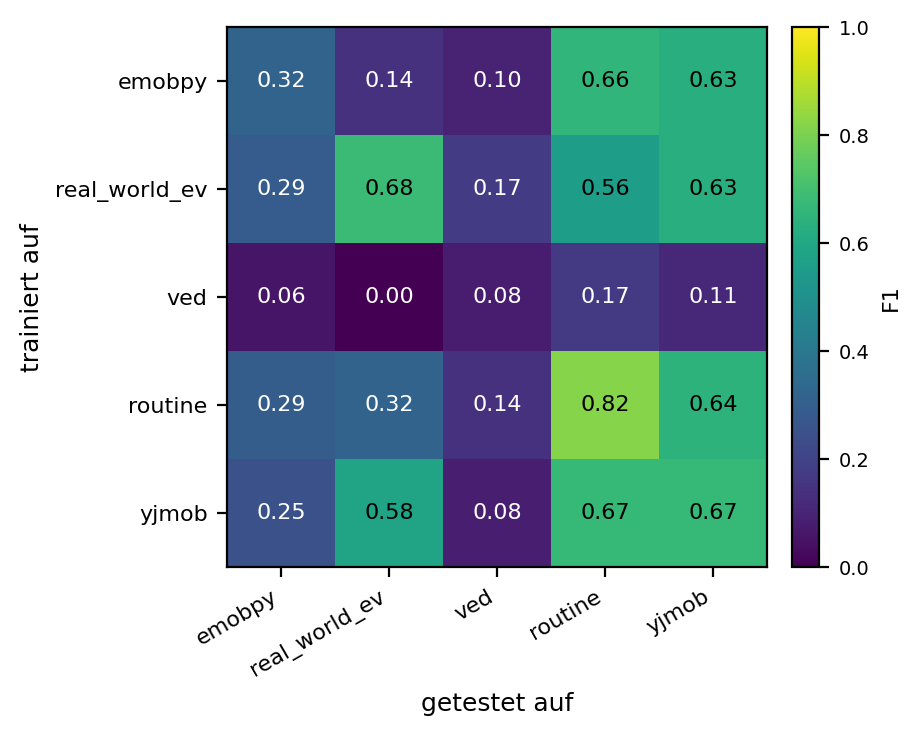
\includegraphics[width=0.8\columnwidth]{cv_f1_5x5.png}
  \captionof{figure}{F1-Werte der 5$\times$5-Kreuzvalidierung}
  \label{fig:cv}
\end{center}

Kernstück der Evaluation ist eine Kreuzvalidierungs-Matrix (\cref{fig:cv}): Jedes Modell wird auf einer Datenquelle trainiert und auf allen getestet. Da Algorithmus und Merkmale konstant bleiben, isoliert das den Effekt der Datenquelle vom Effekt des Algorithmus. Alle Splits erfolgen zeitlich (Vergangenheit~$\rightarrow$~Training, Zukunft~$\rightarrow$~Test), da zufälliges Mischen Informationen aus der Zukunft preisgeben würde. Bewertet wird mit Accuracy, Precision, Recall und F1-Score.



\section{Beitrag und Ausblick}

Die Arbeit adressiert eine in der Forschung bislang wenig beachtete Lücke: die individuelle Prognose des Nutzungsverhaltens über bis zu sieben Tage. Bisherige Arbeiten konzentrieren sich auf Ladeprognosen, aggregiertes Flottenverhalten oder den Ladezustand; das zeitliche Nutzungsmuster einzelner Fahrzeuge bleibt weitgehend unmodelliert -- und wo es betrachtet wird, fehlt meist die saubere Trennung zwischen Daten- und Algorithmuseffekt, die hier im Mittelpunkt steht.

Der konkrete Beitrag umfasst neben dem Modellvergleich und einer Weiterentwicklung des besten Modells die methodische Isolation des Datenbasis-Einflusses über die Kreuzvalidierungs-Matrix sowie kalibrierte Unsicherheitsangaben, die ausweisen, wann einer Prognose vertraut werden kann. Da menschliche Mobilität eine prinzipielle Vorhersagbarkeitsgrenze besitzt~\cite{song2010limits}, ist das Ziel nicht die perfekte Prognose, sondern belastbare, ehrliche Wahrscheinlichkeitsaussagen -- Grundvoraussetzung dafür, dass ein nachgelagertes Energiemanagementsystem sie sinnvoll einsetzen kann.

Als nächste Schritte bieten sich sequenzielle Modelle wie LSTM oder Transformer an, die längere zeitliche Abhängigkeiten direkter modellieren als baumbasierte Verfahren mit manuellen Lag-Merkmalen. Offen bleibt die Übertragbarkeit: Wie gut generalisiert ein auf einem Nutzer trainiertes Modell auf ungesehene Fahrer -- und lässt sich dieser Transfer durch Nutzertypisierung nach Ji~et~al.~\cite{ji2023rethinking} verbessern?

% --- Literatur ---------------------------------------------------------------
\footnotesize
\begin{thebibliography}{9}
\setlength{\itemsep}{0pt}\setlength{\parskip}{0pt}
\bibitem{ji2023rethinking} Ji et al.: \emph{Rethinking the Regularity in
  Mobility Patterns of Personal Vehicle Drivers}. Transactions in GIS, 2023.
\bibitem{gaetemorales2020emobpy} Gaete-Morales et al.: \emph{emobpy: A Tool for
  Generating Battery Electric Vehicle Time Series}. Zenodo, 2020.
\bibitem{pozzato2023fielddata} Pozzato, Allam, Onori: \emph{Analysis and Key
  Findings from Real-World Electric Vehicle Field Data}. Mendeley Data, 2023.
\bibitem{oh2020ved} Oh, LeBlanc, Peng: \emph{Vehicle Energy Dataset (VED)}.
  IEEE T-ITS, 2022.
\bibitem{yabe2024yjmob} Yabe et al.: \emph{YJMob100K: City-scale and
  Longitudinal Dataset of Anonymized Human Mobility Trajectories}. Scientific
  Data, 2024.
\bibitem{breiman2001random} Breiman: \emph{Random Forests}. Machine Learning,
  2001.
\bibitem{song2010limits} Song et al.: \emph{Limits of Predictability in Human
  Mobility}. Science, 2010.
\end{thebibliography}

\end{document}